\documentclass[10pt,a4paper]{article}
\usepackage[utf8]{inputenc}
\usepackage[russian]{babel}
\usepackage[OT1]{fontenc}
\usepackage{amsmath}
\usepackage{amsfonts}
\usepackage{amssymb}
\usepackage{graphicx}
\graphicspath{{Images/}}
\usepackage[left=2cm,right=2cm,top=2cm,bottom=2cm]{geometry}
\usepackage{calc}
\usepackage{wrapfig}
\usepackage{setspace}
\usepackage{indentfirst}
\usepackage{subfigure}
\usepackage{multirow}
\usepackage{longtable}


\title{
Отчет о выполнении лабораторной работы 3.2.5

Вынужденные колебания в электрическом контуре
}

\author{
\vspace{20 cm}
Трунов Владимир, Строчук Андрей. Группа Б01-103}

\begin{document}

\maketitle

\newpage

	\section{Введение}
	
	\textit{Цель работы:} Исследование вынужденных колебаний в электрическом контуре и процессов их установления.
	
	\textit{Оборудование:} генератор звуковой частоты, осциллограф, вольтметр, частотометр, конденсатор, катушка индуктивности, магазин сопротивлений.
	
	\begin{wrapfigure}[9]{r}{0.23\textwidth}
		\vspace{-0.5cm}
		\centering
		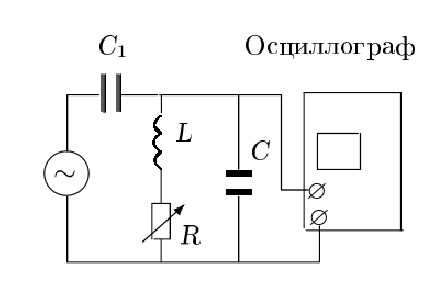
\includegraphics[width = 0.2\textwidth]{schem_of_circuit}
		\caption{Схема исследуемого контура}
		\label{fig:schem_of_circuit}
	\end{wrapfigure}
	
	В работе исследуются вынужденные колебания, возникающие в электрическом контуре (рис \ref{fig:schem_of_circuit}) при подаче на него переменного ЭДС, гармонически изменяющегося со временем. При этом, параметры колебаний будут зависеть как от параметров самого контура -- индуктивности катушки, емкости конденсатора, а также его сопротивления, так и от параметров источника ЭДС -- частоты колебания ЭДС и амплитуды данных колебаний. Основное явление, которое можно наглядным образом наблюдать в подобной системе -- явление резонанса. Резонанс -- явление резкого увеличения амплитуды вынужденных колебаний при частотах источника ЭДС близких к собственной частоте контура.
	
	Кривая, описывающая зависимость амплитуды вынужденных колебаний от частоты источника ЭДС называется резонансной кривой. Первая часть работы будет посвящена исследованию резонансных кривых для контура в двух конфигурациях -- при наличии постоянного сопротивления контура и при его отсутствии.
	
	Исследование резонансных кривых позволит определить \textit{добротность} контура в различных конфигурациях. 
	
	Для этого можно воспользоваться формулой:
	
	\begin{equation}
		Q = \frac{\omega_{0}}{2\Delta \Omega}
		\label{eq:equation_1}
	\end{equation}
	
	где $\omega_{0}$ -- собственная частота контура, $\Delta \Omega = \left|\Omega - \omega_{0} \right|$. 
	
	\begin{wrapfigure}[8]{r}{0.23\textwidth}
		\vspace{-1.5cm}
		\centering
		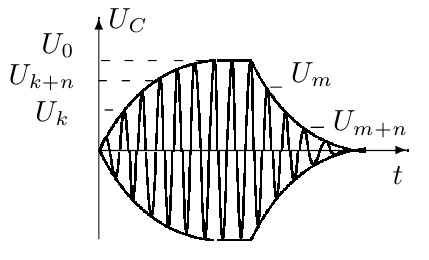
\includegraphics[width = 0.2\textwidth]{graph_of_depence_amplitude}
		\caption{График зависимости амплитуды от времени}
		\label{fig:graph_of_depence_amplitude}
	\end{wrapfigure}\vspace{0.5cm}
	
	Другим же методом, который позволит определить добротность контура является метод исследования процессов установления и затухания колебаний. Данный метод основан на исследовании зависимости амплитуды колебаний в процессе затухания или установления колебаний. График зависимости амплитуды от времени приведен на (рис. \ref{fig:graph_of_depence_amplitude}). В этом случае очень удобно можно получить логарифмический декремент затухания:
	
	\begin{equation}
		\Theta = \frac{1}{n}\ln \left(\frac{U_{0} - U_{k}}{U_{0} - U_{k + n}}\right)
		\label{eq:equation_2}
	\end{equation}
	
	Зная логарифмический декремент затухания, нетрудно выразить добротность контура:
	
	\begin{equation}
		Q = \frac{\pi}{\Theta}
		\label{eq:equation_3}
	\end{equation}
	
	\section{Схема установки}
	\begin{figure}[h!]	
		\begin{center}
			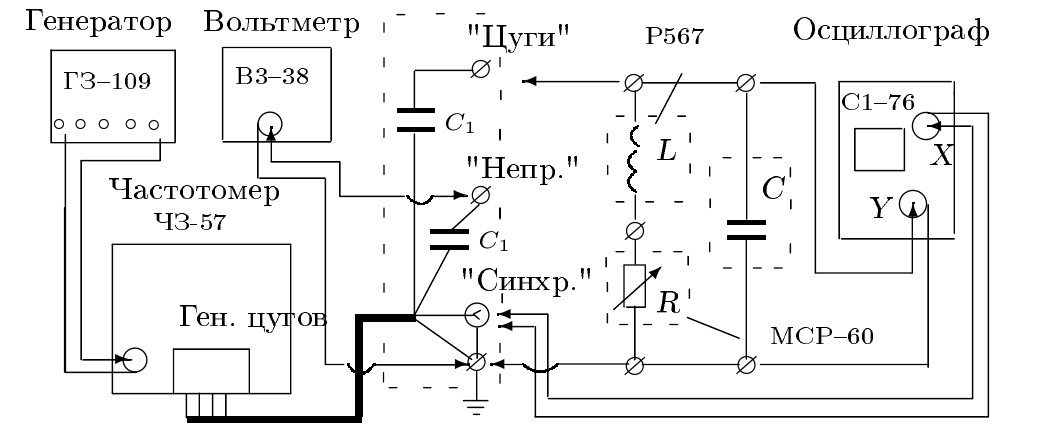
\includegraphics[width = 0.75\textwidth]{schem_of_facility}
			\caption{Схема установки}
			\label{fig:schem_of_facility}
		\end{center}
	\end{figure}
	
	\section{Ход выполнения работы}
	\subsection{Построение резонансных кривых}
	
	\begin{table}[h!]
\centering
\begin{tabular}{|l|l|l|l|l|l|l|l|l|l|l|l|}
    \hline
        \multicolumn{4}{|c|}{$R$ = 0 Oм} & \multicolumn{4}{|c|}{$R$ = 100 Oм} \\ \hline
        {$\nu$, Гц} & {$U$, В} & {$I$, мкА} & {$A$, см} & {$\nu$, Гц} & {$U$, В} & {$I$, мкА} & {$A$, см \\ \hline
       1641 & 31 & 45,9 & 3,80 & 1639 & 10,5 & 46,85 & 2,40 \\ \hline
        1597 & 19,5 & 51,1 & 2,40 & 1528 & 7 & 45,7 & 1,60 \\ \hline
        1592 & 18,2 & 50,87 & 2,20 & 1503 & 6,2 & 45,01 & 1,40 \\ \hline
        1586 & 16,6 & 50,45 & 2,00 & 1473 & 5,5 & 44,15 & 1,20 \\ \hline
        1568 & 13,1 & 49,3 & 1,60 & 1436 & 4,6 & 43,15 & 1,00 \\ \hline
        1543 & 12,9 & 46,75 & 1,20 & 1383 & 3,7 & 41,63 & 0,80 \\ \hline
        1682 & 19,6 & 43,01 & 2,40 & 1797 & 6,9 & 49,15 & 1,60 \\ \hline
        1691 & 17,7 & 43,36 & 2,00 & 1835 & 6,1 & 50,24 & 1,40 \\ \hline
        1722 & 12,7 & 45,05 & 1,60 & 1892 & 5,3 & 51,9 & 1,20 \\ \hline
        1753 & 10 & 46,57 & 1,20 & 1979 & 4,5 & 54,4 & 1,00 \\ \hline
        ~ & ~ & ~ & ~ & 2121 & 3,8 & 58,3 & 0,80 \\ \hline
    \end{tabular}
\caption{Результаты измерения зависимости амплитуды напряжения колебаний в контуре при $R = 0$ Ом и $R = 100$ Ом}
\label{tab:amplitude_measuring}
\end{table}

	\begin{figure}[h!]
		\begin{minipage}{0.49\textwidth}
			\hspace{-0.5cm}
			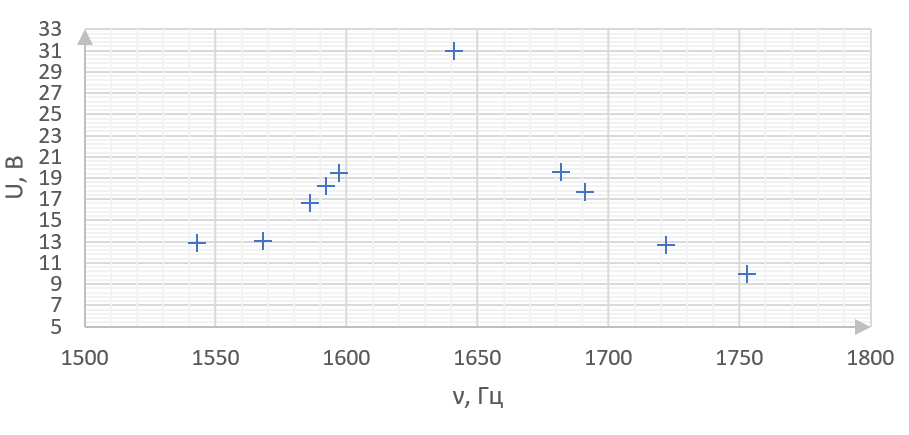
\includegraphics[width = 1.1\textwidth]{GraphR0.png}
			\caption{Резонансная кривая, $R = 0\,$Ом}
			\label{fig:graph_of_depence_amplitude_R=0}
		\end{minipage}
		\hfill
		\begin{minipage}{0.49\textwidth}
			\hspace{-0.5cm}
			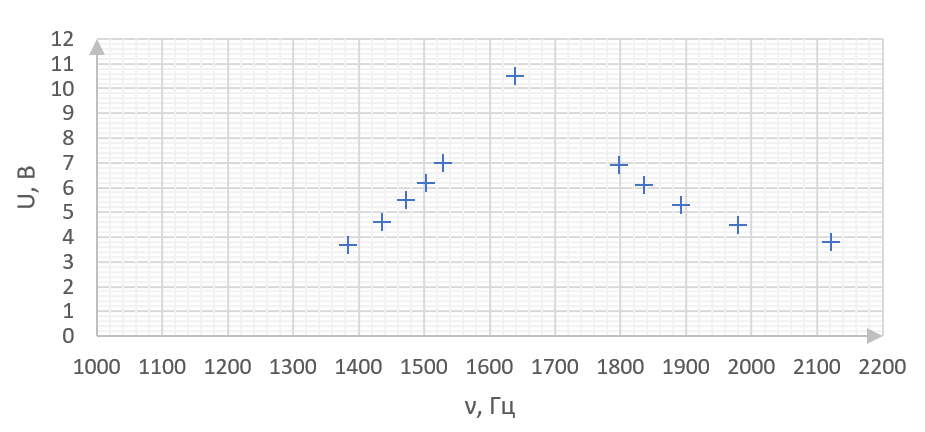
\includegraphics[width = 1.1\textwidth]{GraphR100.png}
			\caption{Резонансная кривая, $R = 100\,$Ом}
			\label{fig:graph_of_depence_amplitude_R=100}
		\end{minipage}
	\end{figure}
    
    Результаты вычисления добротности с использованием формулы (\ref{eq:equation_1}) занесем в таблицу (\ref{tab:Q_from_resonance_curve}) для соответствующих значений $R$
	
	\begin{table}[h!]
\centering
\begin{tabular}{|l|l|l|}
\hline
$R,$ Ом & $Q$ & $\sigma_{Q}$ \\ \hline
0       & 43           & 10,4                      \\ \hline
100     & 10           & 3,7                       \\ \hline
\end{tabular}
\caption{Результаты определения добротности методом исследования резонансных кривых}
\label{tab:Q_from_resonance_curve}
\end{table}
	
	\subsection{Исследование процессов установления и затухания колебаний}
	
	Для определения добротности с помощью исследования процессов установления и затухания вынужденных колебаний необходимо получить зависимость амплитуды вынужденных колебаний в режиме генератора "цуги".
	На основе полученных изображений получим зависимость амплитуд напряжений в процессе установления колебаний (Таблица \ref{tab:Q_measuring_on_grown}) и затухания колебаний (Таблица \ref{tab:Q_measuring_on_decrease})
	
	\begin{table}[h!]
\centering
\begin{tabular}{|l|l|l|l|l|l|l|l|l|l|l|l|l|l|l|l|l|l|l|l|l|}
\hline
 & \multicolumn{8}{|c|}{$R = 0$ Ом} & \multicolumn{4}{|c|}{$R = 100$ Ом} \\ \hline
n            & 1 & 2   & 3   & 4   & 5   & 6   & 12 & 14 & 1  & 2    & 3   & 10  \\ \hline
$U_{n}$, мм & 4 & 16 & 24 & 30 & 36 & 42 & 60 & 66 & 15 & 26 & 35 & 45  \\ \hline
\end{tabular}
\caption{Результаты измерения зависимости амплитуды вынужденных колебаний при их установлении}
\label{tab:Q_measuring_on_grown}
\end{table}	


\begin{table}[h!]
\centering
\begin{tabular}{|l|l|l|l|l|l|l|l|l|l|l|l|l|l|l|l|l|l|l|l|l|}
\hline
& \multicolumn{5}{|c|}{$R = 0$ Ом} & \multicolumn{4}{|c|}{$R = 100$ Ом} \\ \hline
n            & 1 & 4   & 6   & 7  & 9    & 1   & 2   & 3   & 6\\ \hline
$U_{n}$, мм & 8 & 26 & 36 & 40 & 46 & 12 & 20 & 36 & 45\\ \hline
\end{tabular}
\caption{Результаты измерения зависимости амплитуды вынужденных колебаний при их затухании}
\label{tab:Q_measuring_on_decrease}
\end{table}

	\section{Получение добротности контура и определение погрешностей}
	
    \subsection{Исследование установления и затухания колебаний}

Для каждого расчета построим таблицу.

\begin{table}[h!]
	\centering
	\begin{tabular}{|l|l|l|l|l|}
		\hline
		$\mathbf{U_k}$ & $\mathbf{U_{k+n}}$ & $\mathbf{n}$ & $\mathbf{\Theta}$ & $\mathbf{Q}$  \\ \hline
		4      & 24    & 2   & 0,180   & 17,4 \\ \hline
		16    & 36    & 3   & 0,154   & 20,3 \\ \hline
		36   & 60     & 7   & 0,175   & 17,9 \\ \hline
		36   & 66     & 9   & 0,238   & 13,2 \\ \hline
	\end{tabular}
\caption{Расчёт добротности на установлении при $R=0$}
\end{table}

\begin{table}[h!]
	\centering
	\begin{tabular}{|l|l|l|l|l|}
		\hline
		$\mathbf{U_m}$ & $\mathbf{U_{m+n}}$ & $\mathbf{n}$ & $\mathbf{\Theta}$ & $\mathbf{Q}$ \\ \hline
		8         & 26              & 3           & 0,125            & 25         \\ \hline
	    8         & 36              & 5           & 0,126            & 24,8         \\ \hline
		26       & 40              & 3            & 0,128           & 24,6         \\ \hline
		26       & 46              & 5            & 0,121           & 25,9          \\ \hline
	\end{tabular}
\caption{Расчёт добротности на затухании при $R=0$}
\end{table}

\begin{table}[h!]
	\centering
	\begin{tabular}{|l|l|l|l|l|}
		\hline
		$\mathbf{U_k}$ & $\mathbf{U_k+n}$ & $\mathbf{n}$ & $\mathbf{\Theta}$ & $\mathbf{Q}$ \\ \hline
		15         & 26            & 1           &  0,438            & 7,2         \\ \hline
		15         & 35            & 2           & 0.566             & 5,5         \\ \hline
		26         & 45            & 8           & 0.393             & 8,3         \\ \hline
	\end{tabular}
\caption{Расчёт добротности на установлении при $R=100$ Ом}
\end{table}

\begin{table}[h!]
	\centering
	\begin{tabular}{|l|l|l|l|l|}
		\hline
		$\mathbf{U_m}$ & $\mathbf{U_m+n}$ & $\mathbf{n}$ & $\mathbf{\Theta}$ & $\mathbf{Q}$ \\ \hline
		12          & 20            & 1            & 0,268             & 11,7         \\ \hline
		12          & 36            & 2            & 0,612             & 5,13         \\ \hline
		20          & 45            & 5            & 0,652             & 4,82         \\ \hline
	\end{tabular}
\caption{Расчёт добротности на затухании при $R=100$ Ом}
\end{table}

Усредним эти значения:

\begin{equation}\label{key}
	Q_{R=0} = 21.1 \pm 4.6
\end{equation}
\begin{equation}\label{key}
	Q_{R=100} = 7.1 \pm 2.6
\end{equation}

\subsection{Теоретический расчёт}

Определив параметры контура, занесём их в таблицу \ref{2}.

\begin{table}[h]
	\centering
	\begin{tabular}{|l|l|l|}
		\hline
		$\mathbf{\nu}${\bf,  Гц} & $\mathbf{L}${\bf, мГн} & $\mathbf{R}${\bf, Ом} \\ \hline
		50                       & 94.384                 & 23.149                \\ \hline
		500                     & 95.123                 & 23.291                \\ \hline
	\end{tabular}
	\caption{Параметры RLC-контура}
	\label{2}
\end{table}

На их основе рассчистаем $Q$:
\begin{equation}\label{key}
	Q_{R=0} = 42,377 \pm 1,2
\end{equation}
\begin{equation}\label{key}
	Q_{R=100}=7,88 \pm 0.4
\end{equation}
	
	\section{Исследование картины биений вблизи собственной частоты контура}
	
	Для получения картины биений вблизи собственной частоты контура установим на генераторе частоту такую, что графиком сигнала на осциллографе будет синусоида с максимальной амплитудой. Затем, немного отклонив частоту генератора на экране осциллографа получим картину биений, представленную на рисунке 
	
	\begin{figure}[h!]
		\centering
		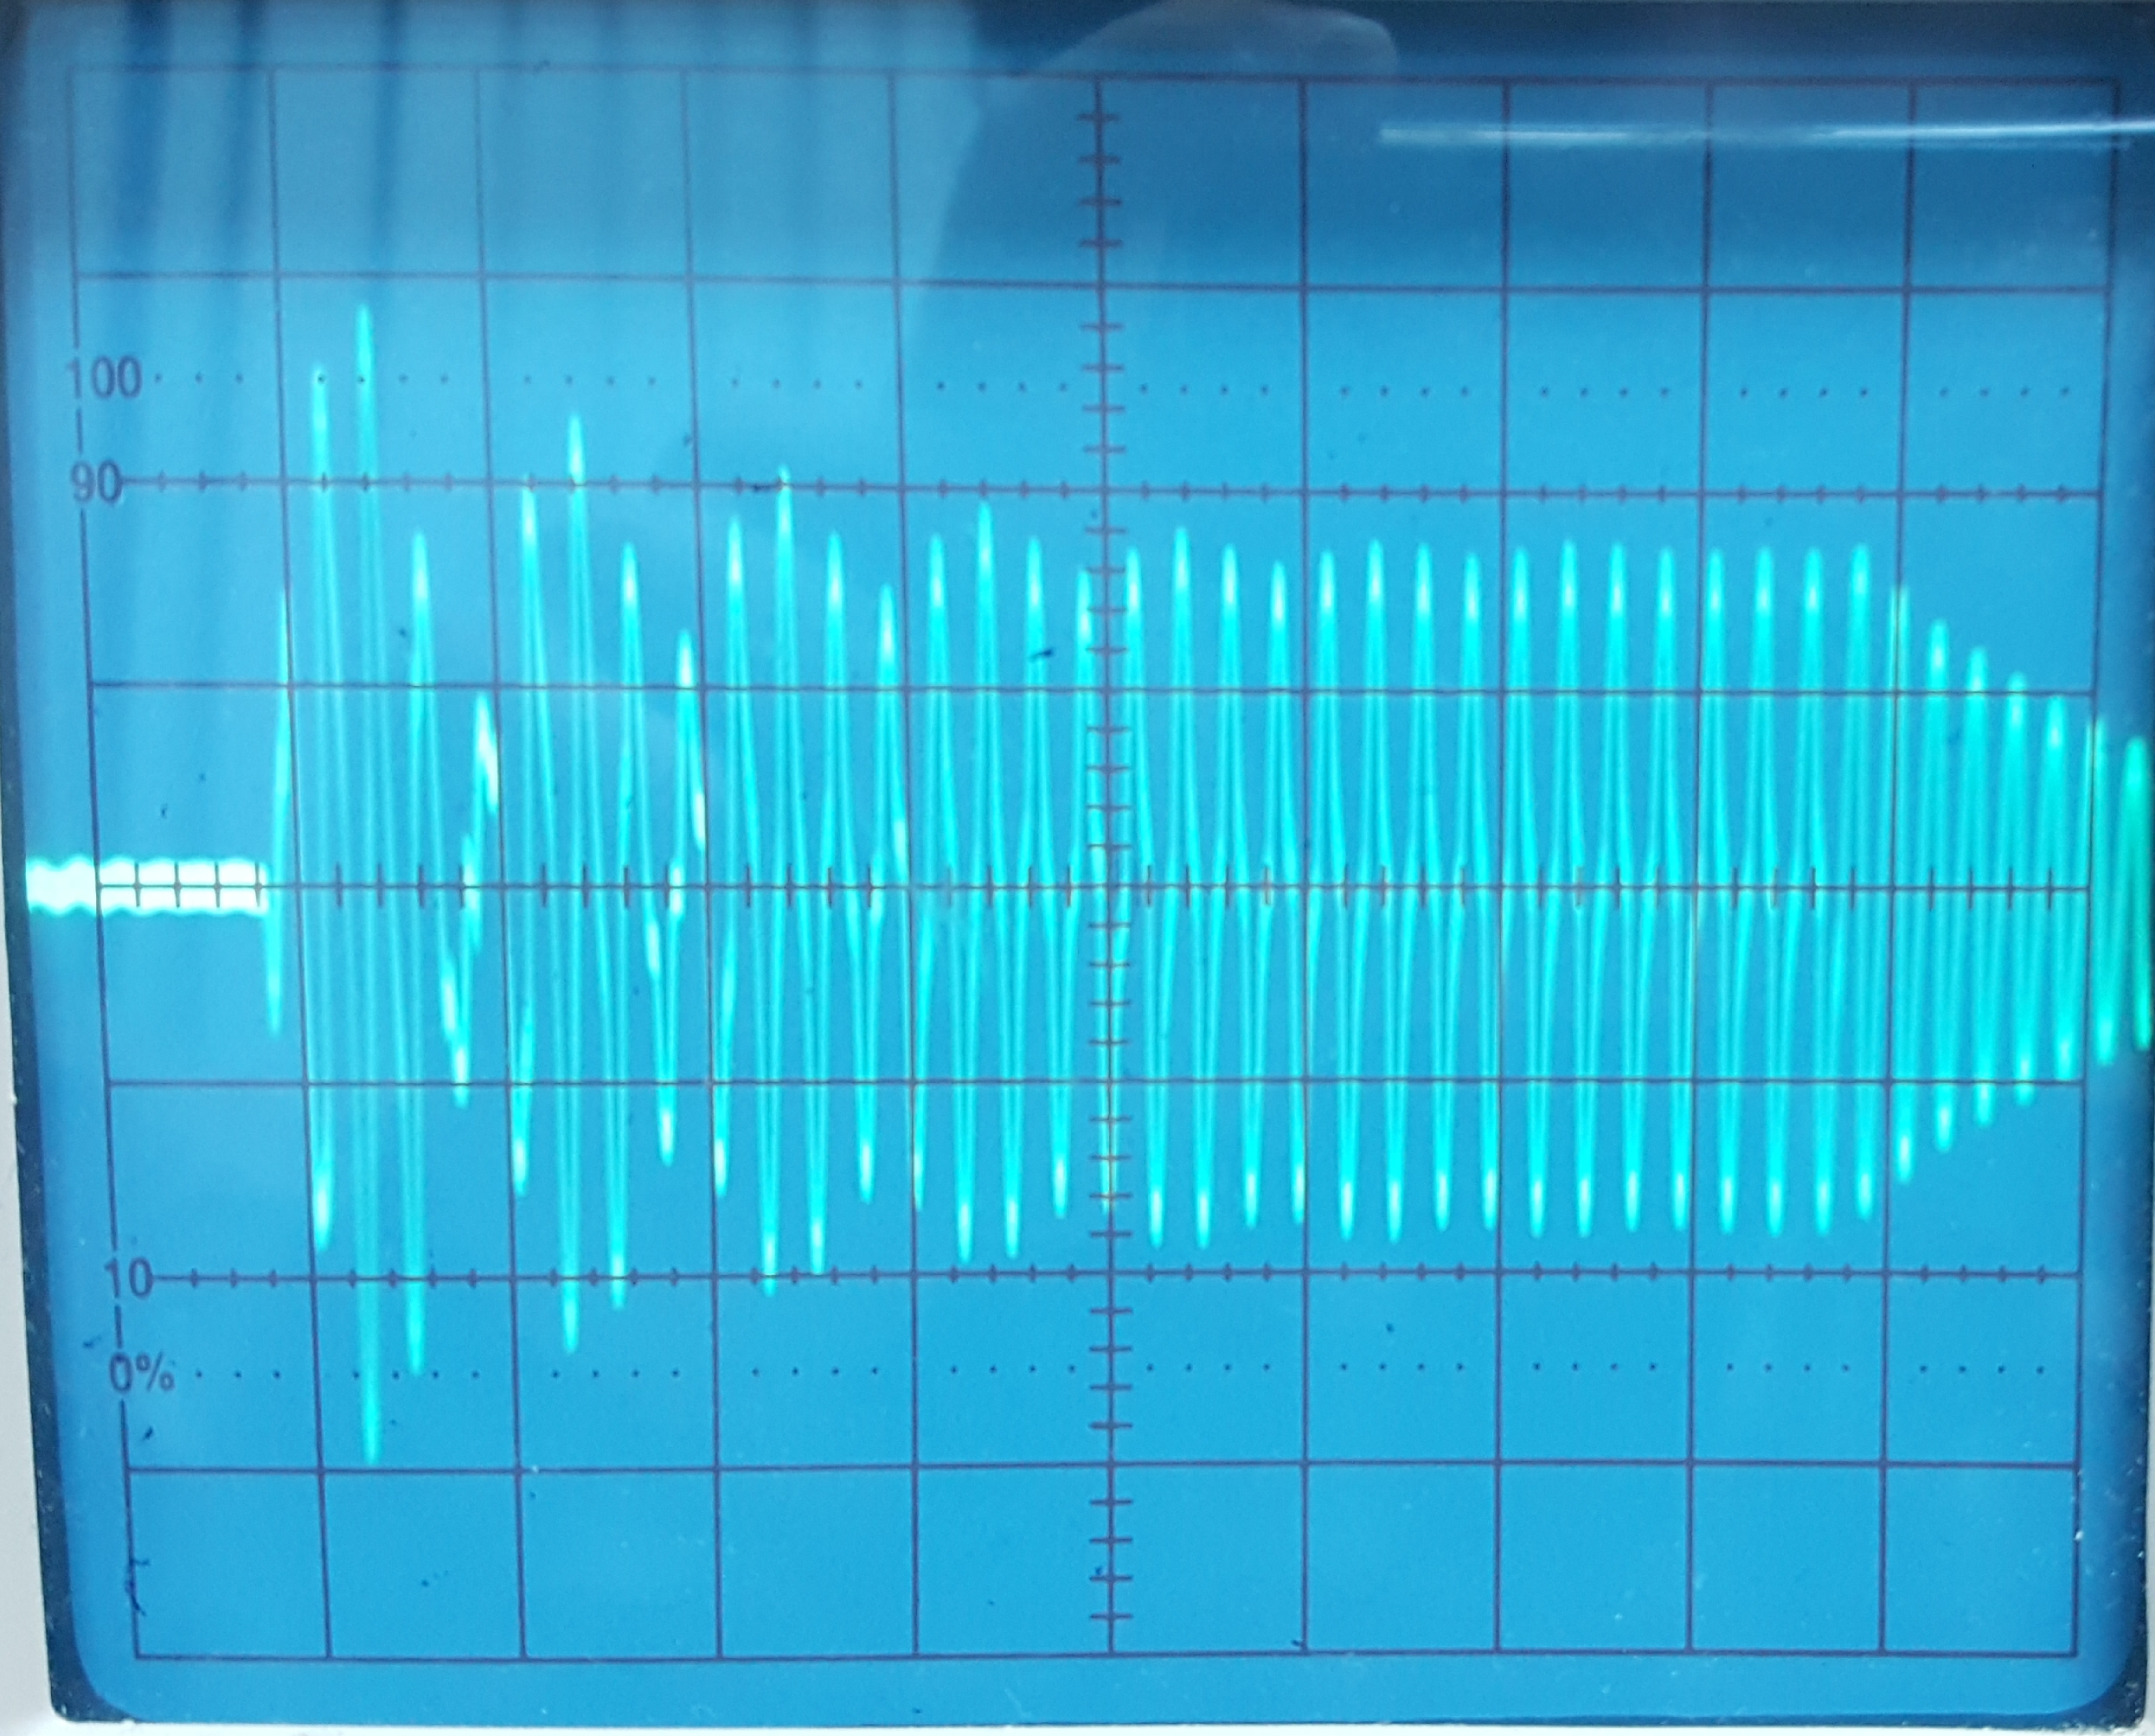
\includegraphics[width = 0.95\textwidth]{beats}
		\caption{Картина биений вблизи собственной частоты контура}
		\label{fig:beats}	
	\end{figure}
	
	\newpage
	
	\section{Итоги}
	
	\begin{enumerate}
		\item В данной работе проведены измерения добротности колебательной системы, представляющей собой электрический колебательный контур, состоящий из последовательно соединенных катушки, резистора переменной емкости (магазин сопротивлений) и конденсатора. Получены значения добротности контура в различных конфигурациях: при $R = 0$ Ом и $R = 100$ Ом.
		\item Проведены измерения погрешностей определения добротности колебательной системы. Установлено, что значения добротности при $R = 100$ Ом согласуются с теоретическими значениями добротности в различных конфигурациях. При $R$ = 0 $Ом$ полученные значения отличаются в 2 раза. Это произошло из-за трудности точного определения показаний осциллографа.
		\item Наибольший вклад в определение погрешности полученных величин внесли статистические (случайные) ошибки, а так же ошибки, связанные с определением величин амплитуд сигнала на экране осциллографа.
		\item Установлено, что при $R = 0$ Ом предпочтительнее проводить измерения добротности методом исследования процессов установления и затухания колебаний, нежели исследованием резонансной кривой. 
		
		Для $R = 100$ Ом недостаточно данных для установления приоритета.
		\item Полученная картина биений соответствует теоретически предсказанной картине.
	\end{enumerate}


	
\end{document}
